\subsection{Vom Plasma ins Netz: Leistungsfluss und Einflüsse}\label{sec:leistungsfluss}
Die Wärmebilanz oben ist als Formelkette hergeleitet. Abbildung~\ref{fig:leistungsfluss} zeigt dieselben Zahlen
als Fluss: Die Breite jedes Bandes ist proportional zur Leistung. Unter den Knoten stehen die Stellgrößen, die den
jeweiligen Wert festlegen. Eine interaktive Fassung, in der man jeden Knoten und jede Stellgröße anklicken kann,
liegt als Webseite vor; das Bild wird mit \texttt{stellarator/einflussgraph.py} erzeugt.

\begin{figure}[H]\centering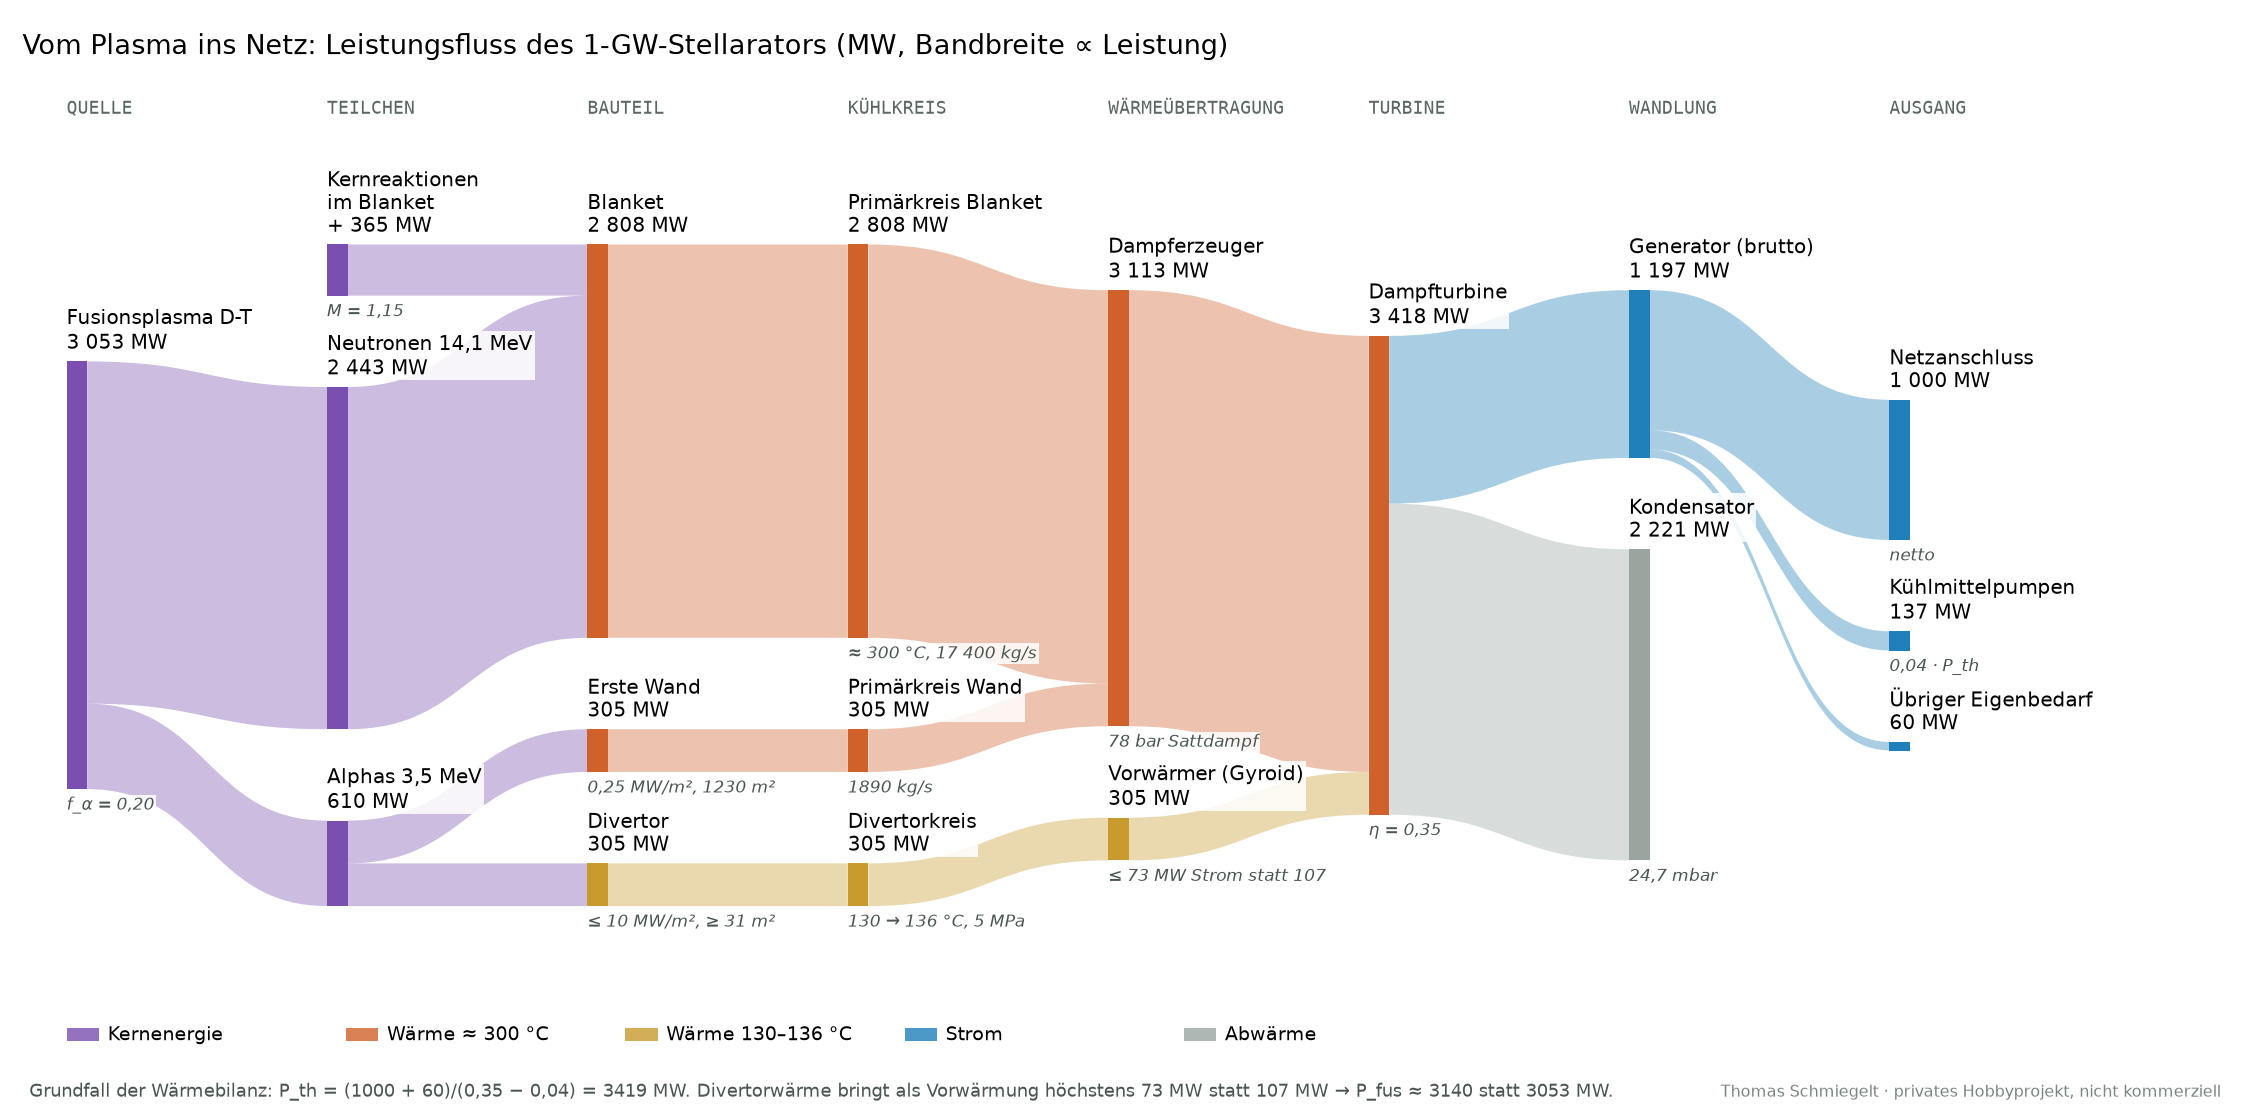
\includegraphics[width=\linewidth]{bilder/einflussgraph.png}
\caption{Leistungsfluss vom Fusionsplasma bis zum Netzanschluss (Grundfall der Wärmebilanz, MW).}\label{fig:leistungsfluss}
\end{figure}
\lesehilfe{Die Bänder fließen von links (Plasma) nach rechts (Netz); die Breite eines Bandes ist
proportional zur Leistung. Die Farben zeigen die Form der Energie: violett Kernenergie, orange Wärme um
\SI{300}{\celsius}, ocker Wärme um \SI{130}{\celsius}, blau Strom, grau Abwärme. Man folgt einem Band, zum Beispiel
Neutronen $\to$ Blanket $\to$ Kühlkreis $\to$ Dampferzeuger $\to$ Turbine $\to$ Generator $\to$ Netz. Die kleinen
kursiven Angaben unter den Knoten sind die Größen, die den jeweiligen Wert bestimmen. Das breite graue Band zum
Kondensator ist der größte Verlust.}


\paragraph{Lesart.} Von \SI{3053}{MW} Fusionsleistung kommen \SI{1000}{MW} im Netz an, knapp ein Drittel. Den
größten Verlust erleidet die Leistung nicht im Kraftwerksteil mit Plasma und Magneten, sondern in der Turbine: Der
Kondensator gibt \SI{2223}{MW} als Abwärme ab. Das ist bei jedem Dampfkraftwerk so und folgt aus der
Frischdampftemperatur. Die Kette hat drei Stellen, an denen der Entwurf den Wirkungsgrad direkt beeinflusst:
\begin{itemize}
\item die \textbf{Kühlmitteltemperatur} von Blanket und Wand (etwa \SI{300}{\celsius}). Sie setzt den
  Frischdampfdruck von \SI{78}{bar} und damit $\eta=0{,}35$;
\item die \textbf{Divertortemperatur} (\SI{136}{\celsius}). Sie macht aus \SI{305}{MW} Wärme nur Vorwärmung, die
  höchstens \SI{73}{MW} Strom bringt (Abschnitt~\ref{sec:vorwaermer});
\item die \textbf{Druckverluste} in Kanälen und Tauschern. Sie gehen über die Pumpen (\SI{137}{MW}) direkt vom
  Netto ab.
\end{itemize}
Die Stellgrößen der Physik ($f_\alpha$, $M$) bestimmen, wie viel Fusionsleistung für \SI{1}{GW} netto nötig ist,
nicht den Wirkungsgrad danach.

\IfFileExists{bauteile_de.tex}{\subsection{Die Bauteile der Kette}\label{sec:bauteile}
Dieser Abschnitt erklärt die Bauteile vom Plasma bis ins Netz in einfachen Worten. Allgemeines Fachwissen ist belegt; Zahlen mit dem Hinweis „Projekt“ sind Annahmen oder Ergebnisse dieser Auslegung.

\paragraph{1. Fusionsplasma und Magnetspulen.} Im Plasma verschmelzen Deuterium und Tritium (D-T) bei rund 150 Millionen \si{\celsius} \cite{bt_iter_fusion}. So heißes Gas berührt keine Wand. Magnetfelder halten es in der Schwebe. Ein Stellarator formt dieses Feld allein mit verdrehten Außenspulen und treibt keinen Strom durch das Plasma. Er läuft daher von Natur aus im Dauerbetrieb, braucht aber stärkere Magnete als ein Tokamak \cite{bt_stellarator}. Große Anlagen wie Wendelstein~7-X nutzen supraleitende Spulen, die flüssiges Helium auf etwa \SI{4}{K} kühlt \cite{bt_w7x_en}. Dafür braucht es eine Kälteanlage. Projekt: Das Plasma liefert $P_\text{fus} = \SI{3053}{MW}$ (mit Vorwärmer-Korrektur etwa \SI{3140}{MW}). Offen: die Kräfte zwischen den Spulen sind etwa 1000-mal so groß wie bei W7-X, und die Stützstruktur ist noch nicht gelöst.

\paragraph{2. Neutronen und Alphateilchen.} Jede D-T-Fusion setzt \SI{17,6}{MeV} frei. Etwa \SI{80}{\percent} trägt das Neutron, den Rest das Heliumkern-Teilchen (Alpha) \cite{bt_dtfusion,bt_fusionpower}. Das Neutron hat keine Ladung. Es verlässt das Magnetfeld und gibt seine Energie in der Wand und im Blanket ab. Das Alphateilchen bleibt im Plasma und heizt es \cite{bt_tokamak}. Projekt: $f_\alpha = 0{,}2$ (genau $3{,}52/17{,}59$). Annahme: Die Alpha-Leistung verlässt das Plasma je zur Hälfte als Strahlung auf die Erstwand und als Teilchenstrom auf den Divertor ($f_\text{div} = 0{,}5$). Offen ist diese Aufteilung; sie hängt vom realen Plasma ab.

\paragraph{3. Erste Wand.} Die erste Wand ist die Verkleidung, die dem Plasma zugewandt ist. Sie schützt die Spulen und fängt Wärme und Strahlung ab \cite{bt_firstwall}. Bei ITER sitzt sie auf abnehmbaren Paneelen, und der Panzer wechselt von Beryllium zu Wolfram \cite{bt_iter_blanket}. Wolfram hat den höchsten Schmelzpunkt aller Metalle, wird aber spröde \cite{bt_firstwall}. Projekt: Die Wand fängt \SI{305}{MW} Strahlung auf. Das sind \SI{0,25}{MW/m^2} auf \SI{1230}{m^2}. Die Kühlkanäle sind für \SI{0,5}{MW/m^2} ausgelegt, also mit Faktor 2 Reserve. Das Kühlwasser (\SI{1890}{kg/s}) erwärmt sich um \SI{30}{K}. Offen: Neutronenschäden am Wandmaterial; sie sind hier nicht untersucht.

\paragraph{4. Blanket.} Das Blanket sitzt hinter der ersten Wand. Es hat drei Aufgaben: Es bremst die Neutronen ab und wandelt ihre Energie in Wärme. Es erbrütet Tritium, indem Neutronen auf Lithium treffen. Es schirmt die Spulen ab \cite{bt_breeding,bt_iter_blanket}. Tritium kommt in der Natur kaum vor; nur das Blanket kann es liefern \cite{bt_breeding}. Blei oder Beryllium vermehren die Neutronen (Multiplikation) \cite{bt_breeding}. Projekt: $M = 1{,}15$ (Annahme). Das Blanket führt \SI{2808}{MW} ab, mit \SI{17400}{kg/s} Druckwasser bei etwa \SI{300}{\celsius} und $\Delta T = \SI{30}{K}$. Das EU-DEMO-Konzept WCLL (Wasser, Blei-Lithium) zielt auf diese Bedingungen \cite{arena2023}. Offen: Kann das Blanket zugleich \SI{2,8}{GW} abführen und genug Tritium erbrüten?

\paragraph{5. Divertor.} Der Divertor lenkt Teilchen und Wärme, die aus dem Plasma entweichen, entlang offener Feldlinien auf gesonderte Platten \cite{bt_divertor}. Er führt Asche und Verunreinigungen ab und hält das Plasma sauber \cite{bt_iter_divertor}. Die Asche besteht vor allem aus Helium, das die D-T-Fusion erzeugt \cite{bt_dtfusion}; Vakuumpumpen saugen es ab. Beim ITER-Divertor liegt die Flächenlast stetig bei etwa \SI{10}{MW/m^2}, in langsamen Spitzen bis \SI{20}{MW/m^2} \cite{bt_iter_divertor}. Projekt: \SI{305}{MW} auf mindestens \SI{31}{m^2} bei \SI{10}{MW/m^2}. Er wird kalt gekühlt (Wasser \SI{130}{\celsius} rein, \SI{136}{\celsius} raus, \SI{5}{MPa}), wie beim EU-DEMO \cite{you2022}. Das Projekt setzt dafür eine Kupferlegierung an. Offen: die Lebensdauer unter dieser Last.

\paragraph{6. Primärkühlkreise.} Die Kühlkreise von Blanket und Wand führen die Wärme heraus. Sie arbeiten mit Druckwasser wie im Druckwasserreaktor. Der hohe Druck hält das Wasser flüssig, obwohl es weit über \SI{100}{\celsius} heiß ist \cite{bt_pwr}. Projekt: etwa \SI{300}{\celsius}, $\Delta T = \SI{30}{K}$, \SI{17400}{kg/s} durch das Blanket und \SI{1890}{kg/s} durch die Wand. Der Druck von rund \SI{16}{MPa} ist eine Annahme. Auch die Wahl dieser Bedingungen ist eine Projekt-Entscheidung: Sie erlaubt eine Turbine aus einem Druckwasserreaktor. Offen: Die Leitungen müssen durch die engen Spulenspalte. Die Rechnung zeigt, dass sie dort reichlich Platz haben (mehr als Faktor 10 Reserve).

\paragraph{7. Dampferzeuger.} Der Dampferzeuger ist ein Wärmetauscher. Heißes Primärwasser fließt durch viele dünne Rohre, außen siedet Wasser des Sekundärkreises zu Dampf \cite{bt_steamgen}. Die Rohrwände trennen die Kreise, sodass Primärwasser nicht in die Turbine gelangt \cite{bt_steamgen,bt_pwr}. Das Projekt nimmt an, dass das Primärwasser Tritium oder Aktivierung tragen kann. Projekt: Frischdampf mit \SI{78}{bar}, gesättigt, \SI{2443}{kg/s}. Das sind die Werte des EPR \cite{epr_en}. Der Dampf ist gesättigt wie im Druckwasserreaktor; dafür setzt das Projekt $\eta = 0{,}35$ an (Annahme). Offen: Tritium kann durch die Rohrwand wandern; das ist nicht untersucht.

\paragraph{8. Divertor-Vorwärmer.} Die Divertorwärme fällt bei nur etwa \SI{130}{\celsius} an. Das reicht nicht für Dampf, wohl aber zum Vorwärmen des Speisewassers. Das spart Anzapfdampf, der dann in der Turbine Arbeit leistet. Projekt: Der Gyroid-Tauscher, eine gedruckte Wand mit gewundenen Kanälen, soll die \SI{305}{MW} übertragen. Ergebnis der Rechnung: Der Vorwärmer bringt höchstens \SI{73}{MW} Strom, und zwar nur ohne Temperaturannäherung und ohne Pumpen. Zum Vergleich: \SI{107}{MW} wären \SI{35}{\percent} von \SI{305}{MW}. Geht die Wärme ganz verloren, steigt die nötige Fusionsleistung um \SI{10}{\percent}. Offen: Die Korrelationen stammen aus Versuchen im kleinen Maßstab.

\paragraph{9. Dampfturbine.} Die Turbine lässt den Dampf in vielen Stufen entspannen und wandelt Druck in Drehung um \cite{bt_turbine}. Mit Zwischenüberhitzung geht der Dampf nach der Hochdruckstufe zurück in einen Erhitzer und strömt dann weiter. Das bringt mehr Arbeit und weniger Tropfen in den letzten Schaufeln \cite{bt_turbine}. Projekt: Wärme $P_\text{th} = \SI{3419}{MW}$, Wirkungsgrad $\eta = 0{,}35$, also brutto \SI{1197}{MW}. Vergleich: Isar~2 hatte \SI{3950}{MW} thermisch und \SI{1485}{MW} brutto; eine Turbine dieser Klasse reicht. Annahme: Eine solche Turbine ist verfügbar. Offen: ob eine stillgelegte Turbine erhältlich ist.

\paragraph{10. Kondensator und Kühlturm.} Der Kondensator kühlt den Abdampf zu Wasser. Er arbeitet im Unterdruck, damit die Turbine mehr Energie entnimmt \cite{bt_condenser}. Die frei werdende Wärme muss weg: Ein Nasskühlturm gibt sie ab, indem ein Teil des Wassers verdunstet \cite{bt_cooling}. Projekt: \SI{2223}{MW} Abwärme bei \SI{24,7}{mbar} (\SI{20,9}{\celsius}). Das ist fast das Doppelte der Strom-Leistung. Das ist bei jedem Dampfkraftwerk so. Offen: Standort und Wasserbedarf des Kühlturms; das Projekt hat sie nicht bestimmt.

\paragraph{11. Generator.} Der Generator wandelt die Drehung der Turbinenwelle in Strom. Er nutzt die elektromagnetische Induktion: Ein bewegtes Magnetfeld erzeugt in Wicklungen eine Spannung \cite{bt_generator}. Kraftwerke setzen Synchrongeneratoren ein, die mit dem Netz im Takt laufen müssen \cite{bt_generator,bt_turbine}. Projekt: Er erzeugt brutto \SI{1197}{MW} Wechselstrom. Davon gehen \SI{197}{MW} an den Eigenbedarf. Die Bilanz rechnet nur mit dem Gesamtwirkungsgrad $\eta$; ein Generatorwirkungsgrad steht nicht gesondert darin. Offen: Auswahl und Größe.

\paragraph{12. Eigenbedarf.} Die Anlage verbraucht einen Teil ihres Stroms selbst. Projekt: Die Kühlmittelpumpen brauchen \SI{137}{MW} ($0{,}04\,P_\text{th}$, Annahme). Dazu kommen \SI{60}{MW} für den übrigen Eigenbedarf: die Kälteanlage der Spulen, die Tritiumanlage und Gebäude. Die Kälteanlage hält die Spulen auf wenigen Kelvin \cite{bt_w7x_en}. Die Tritiumanlage soll Tritium aus Blanket und Abgas gewinnen und dem Plasma wieder zuführen (Beschreibung des Projekts, nicht belegt). Der Wert für den Rest ist eine Annahme; für die Erstwandkanäle allein rechnet das Projekt nur mit etwa \SI{8}{MW} Pumpleistung. Offen: Der Gesamtwert von \SI{197}{MW} ist nicht aus Einzelteilen aufgebaut.

\paragraph{13. Transformator und Netzanschluss.} Ein Transformator hebt die Generatorspannung an, denn bei hoher Spannung fließt für dieselbe Leistung weniger Strom, und die Leitungen verlieren weniger Wärme \cite{bt_transformer}. Das Hochspannungsnetz nimmt den Strom dann auf. Projekt: Ins Netz gehen netto \SI{1000}{MW}. Das ist die Vorgabe, aus der die ganze Kette rückwärts gerechnet wurde. Verluste im Transformator sind in der Bilanz nicht angesetzt. Offen: Netzanschlusspunkt und Auslegung.
}{}
